\section{Food problems and their impact on childhood }
One of the main problems of modern society is the one related to nutrition. Nutrition was changed a lot in history thanks to the industrial development that allowed the massive production of foods that in the past were produced only by hand (and with high costs) and thanks also to scientific progresses that allowed the discovery of food conservation and their elaboration to obtain new kinds of food that are more suitable to our need. Montignac \cite{Lastoriadell'alimentazionedell'uomo.} also identifies other causes that brings the concept of "nutrition" to assume the current meaning, for example the habits evolution and the female emancipation that have changed the ancient vision of women as "landladies" and that have promoted the progression of the "ready meals" industry and therefore of pre-cocked and packaged meals that today are consumed increasingly. However, the main phenomenon that has taken place in our era is the one related to the globalization and standardization of destabilized north american eating habits that has promoted the global growth of fast-food, indicated by WHO (World Health Organization) as a "pandemic" since 1997 given its extraordinary expansion that carried also a lot of other problems.\\
Childhood obesity is surely one of the clearest examples of these diet's changes of the new millennium.
According to a seminar held by CB Ebbeling, DB Pawlak and DS Ludwig \cite{Childhoodobesity} childhood obesity is a phenomenon that has had a great increase in all the world in the last twenty years, as we can see from this diagram.\clearpage
\begin{figure}[H]
\centering
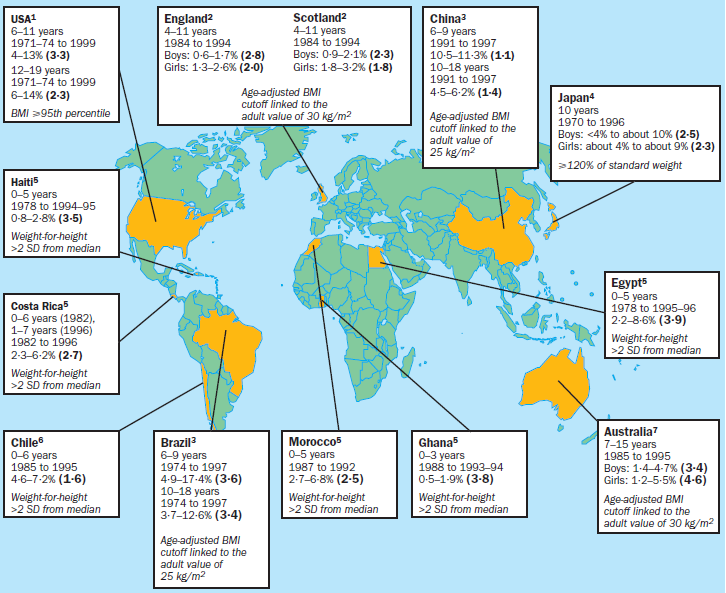
\includegraphics[width=13cm, height=10cm]{immagini/obesity.png}
\caption{Childhood obesity diagram}\label{fig:obesity}
\end{figure}
Historically, a fat child was seen as healthy because he was likely to survive better to illnesses and infections; however, excessive fatness has become one of the most diffused health problem in children. The three experts have underlined how the problem is most common in developed and industrialized nations in which diet has changed radically favoring foods containing saturated and trans fat and with high glycemic index, typical of fast-food in which also bigger portions are served. Moreover, these foods are also poor of fibers, micronutrients and antioxidants that the body needs for a correct functioning of metabolism. The excessive consuming of these foods brings the child to have health problems such as heart diseases, vascular disorders, hypertension, chronic inflammations and diabetes of type 2, illness that in the past was not present in teenagers, but that now has had a rapid spread.\linebreak 

Another important problem that affects the food safety of children is represented by allergies.
According to the data collected by AM Branum and SL Lukacs \cite{FoodallergyUSchildren} it is possible to observe an increasing in cases of all kinds of food allergies including milk, eggs, peanuts, tree nuts, fish, shellfish, soy and wheat of around the 18 per cent on individuals under the age of 18 from the 1997 onwards in US (but we have reasons to believe that this can also be found in all the industrialized world). Reactions to these foods may vary from small diseases to anaphylactic shock that, in severe cases, could lead to death.
The researches have also underlined how, in the same period analyzed previously, there was also an increasing of hospital discharges (clearly after an hospitalization) due to allergic reactions as we can see from this barplot.
\begin{figure}[H]
\centering
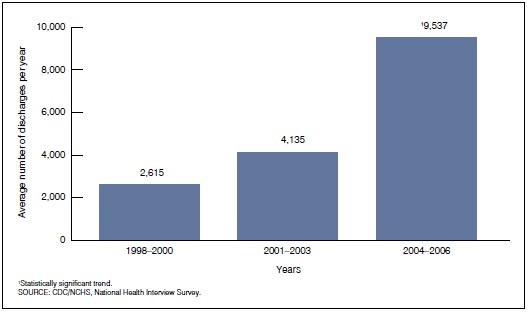
\includegraphics[width=10cm, height=7cm]{immagini/allergybarplot.png}
\caption{Allergy hospital discharges barplot}\label{fig:allergybarplot}
\end{figure}
All these problems that have been reinforced in recent years, lead us to think that it is necessary to support nutrition education and to make it a fundamental thing during childhood and adolescence, in order to empower everyone to a correct care of their health.

\section{Virtual Reality}
"Virtual Reality is electronic simulations of environments experienced via head mounted eye goggles and wired clothing enabling the end user to interact in realistic three-dimensional situations." (Coates, 1992)\\
We can define it using two variables: vividness, richness of an environments representation, and interactivity, extend to which a user can modify form and content of a mediated environment. The vividness is composed by sensory breadth, which refers to the number of sensory dimensions simultaneously presented, and sensory depth, which refers to the resolution within each of these perceptual channels; the interactivity instead is formed by speed, which refers to the rate at which input can be assimilated into the mediated environment, range, which refers to the number of possibilities for action at any given time and mapping, which refers to the ability of a system to map its controls to changes in the mediated environment in a natural and predictable manner.\cite{StefanSeipel} All of them, combined together, influence the telepresence that refers to a set of technologies which allow a user to feel as if he was present at a place different from his true location. So a "virtual reality" is defined as a real or simulated environment in which a perceiver experiences telepresence.\cite{JonathanSteuer}\\
\begin{figure}[H]
\centering
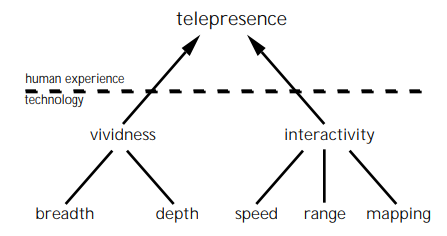
\includegraphics[width=8cm, height=5cm]{immagini/telepresence.png}
\caption{Telepresence influencing variables}\label{fig:telepresence}
\end{figure}
We focus our project on Wearable Immersive Virtual Reality (WIVR). Immersive is the term that refers to the degree to which a virtual environment submerges the perceptual system of the user in computer-generated stimuli. The more the system captivates the sense and blocks out stimuli from the physical world the more the system is considered immersive.\cite{BioccaDelaney} Wearable indicates that the virtual environment is displayed in specialized small screen: we use a binocular head mounted displays (HMD) which allows to reach a fully immersive experience as we can see from this taxonomy by Muhanna \cite{Muhanna}.
\begin{figure}[H]
\centering
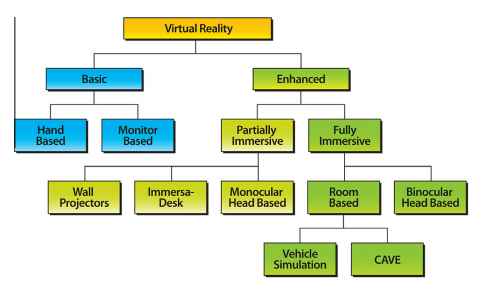
\includegraphics[width=10cm, height=7cm]{immagini/vrtaxonomy.png}
\caption{Virtual Reality taxonomy}\label{fig:vrtaxonomy}
\end{figure}
The HMD "trick" our brain using the principle of stereoscopic vision to simulate the perception of depth and to create 3D images and spaces, the VR has to generate two different images one for each eyes. The lenses of the visor augments the eyes in such a way we can converge the two scenes to obtain only one but that seems to be in the 3 dimensions space. Finally it can track the head movement so when we move it the space updates. 
\begin{figure}[H]
\centering
\begin{minipage}[c]{.40\textwidth}
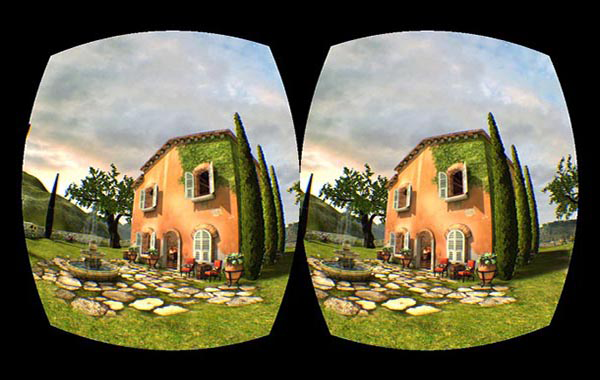
\includegraphics[width=1\textwidth]{immagini/immaginedoppia.png}
\end{minipage}%
\hspace{10mm}%
\begin{minipage}[c]{.40\textwidth}
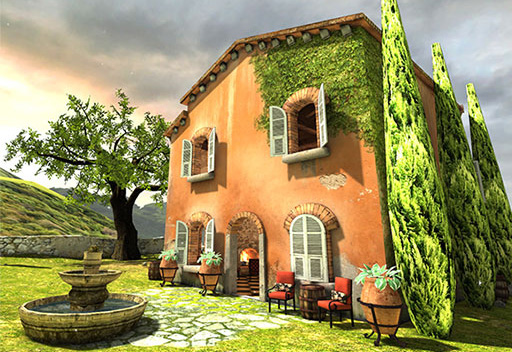
\includegraphics[width=1\textwidth]{immagini/immaginesingola.png}
\end{minipage}
\caption{Stereoscopic image and the correspondent 3D image}\label{fig:vrimages}
\end{figure}
Nowadays HMD are very popular and the costs are in a very big range from a cheap one, like Google Cardboard \cite{Cardboard}, to a more expensive one, like Samsung Gear VR \cite{Gear}, so the VR is for everyone. The VR is also used in a lot of different sectors as we can see in the following graph representing the investments in the 2015 taken from Digi-Capital \cite{DigiCapital}.
\begin{figure}[H]
\centering
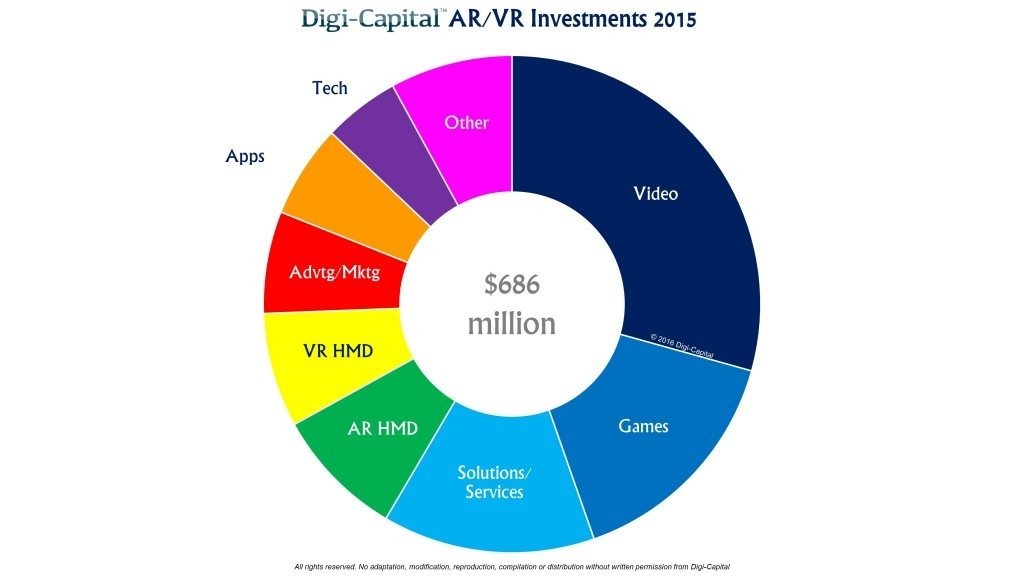
\includegraphics[width=15cm, height=7cm]{immagini/vrsectors.png}
\caption{Virtual Reality investments sectors}\label{fig:investments}
\end{figure}

\section{Touch screen}
Touch screen technology is something we have had for a longer time one can think. The first touch screen device in fact was a radar built in capacitive way and dates back to around 1966. Its invention is due to E. A. Johnson and it works using a sheet of conductive, transparent material with a small current flowing on it. The central computer computes the current at each of the four corners, and when an objects touches the screen, a capacitor is formed between it and the platform and measuring again, the current on the corners the computer is able to approximately compute the point in which there was the touch.\\
At first this technology was abandoned, then in the first 2000s it was used on BlackBerry devices, but the major explosion of touch screen devices is in the 2007, when Apple releases the first iPhone. \cite{Infante}
From that point on, touch screen devices become increasingly used (as we can see from the graph below related to phones) and have had an explosive growth due to their main characteristic: the human computer interaction.
\begin{figure}[H]
\centering
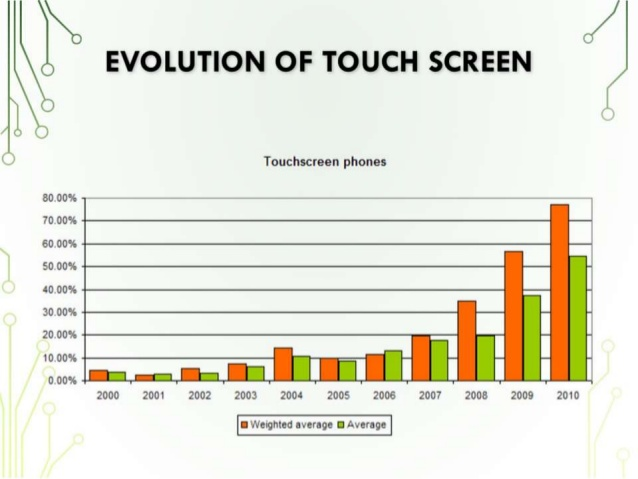
\includegraphics[width=12cm, height=9cm]{immagini/evolutouch.jpg}
\caption{Evolution of touch screen}\label{fig:evolutouch}
\end{figure}
This interaction could be exploited by the fact that the user could touch directly what he wants without recurring to a third element (like a mouse) and this is particularly appealing because it makes the interaction more intuitive and allows a better usability of the system that is one of the main reasons of the success of this kind of devices. Moreover this improved usability will result in a easier training of people that learns faster and better with reduced costs due to the fact that this technology has grown a lot in recent years and it is no longer excessively expensive and resource-hungry \cite{Creed}.

\section{Neurodevelopmental Disorder}
The term neurodevelopmental disorder, NDD, contains within it all the conditions that are caused by a dysfunction of a part of the brain or nervous system that show some symptoms in the physical and psychological development of the child \cite{EPA}. Among the most common diseases we find Autism, ASD, attention deficit and hyperactivity, ADHD, and Down syndrome \cite{APA}. Children who suffer from these syndromes need help in developing cognitive abilities such as attention and language, social skills such as the ability to relate to others and personal and domestic autonomy skills. Dr. Dorothy Strickland, Department of Computer Science of North Carolina State University, in her treatise on the study of a VR application for autistic children \cite{Dorothy}, states that among the great benefits that can be found are: control on input stimuli, small changes to reach a generalization, safe learning situations, personalized treatment and learning with minimal human interference. In recent years there has been an increase in interest in the use of VR especially in the field of NDDs, \cite{Yufang} and \cite{Garzotto}, as, as stated in \cite{Strickland}, both the strength and limitations of Virtual Reality seem to adapt good for the needs that the learning tools for this type of disability require.\\
\\
As for the spread of these diseases take for example the autism on which there are no certain data, but there is agreement on the fact that the phenomenon is growing. According to the World Health Organization (WHO), ASD affects one child in 160 and recent estimates by the Cdc (Center for Disease Control) indicate that 3 million people are affected by this disorder in the US and about 60 million in world. According to estimates gathered by World Atlas, it would be Japan and Great Britain where autistic disorders occur more often.
\begin{figure}[H]
\centering
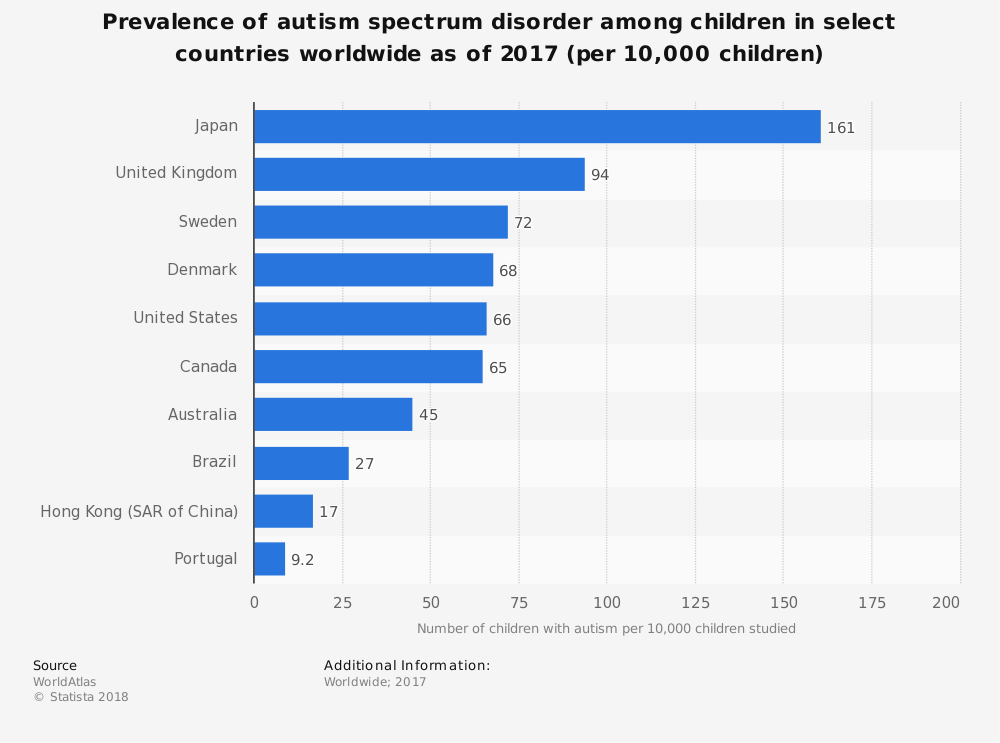
\includegraphics[width=15cm, height=10cm]{immagini/autismo.png}
\caption{Autism diffusion by World Atlas}\label{fig:autism}
\end{figure}

\section{Participatory Design and Therapy}
Over the past six decades, designer have been moving increasingly closer to the future users of what they design. In particular, design is becoming something that is more and more related to what the user needs, this imply the necessity of the collaboration between the experts in field (designers) and the final users (that are usually not experts) leading to what is now called co-design process.\\
The historic user-centered approach, in which designers thought as the user as final objective of their studies, but considered him as a passive entity, have been gradually substituted by the co-design process since the 1970s because people have been giving more importance to activities in which their opinion is required.
\begin{figure}[H]
\centering
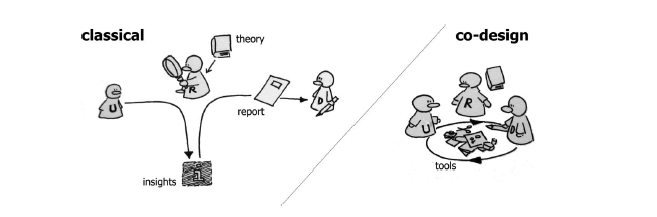
\includegraphics[width=16cm, height=5cm]{immagini/codesign.png}
\caption{Classical approach vs codesign approach}\label{fig:codesign}
\end{figure}
In the classical approach in fact, as we can see in the image above, there were different entities that collaborates to the final design of the product, but the user was considered a passive object of study: researches brings knowledge from theory and developed some more through the observation and interviews. Designer then apply this knowledge to conceptualize the final product. 
In co-creation approach, on the other hand, the roles get mixed-up: the user is involved as "expert of his/her experience" and plays a large role in the knowledge development idea generation and concept development \cite{Elizabeth}.\\
In the field of NDD, this could lead to multiple benefits: in particular, the target user perspective is taken into account since the early design phase and this allow to create something ad-hoc for this kind of people (for example the usage of simple words in explanations, the usage of certain kind of graphic stuffs and so on) and for the participants point of view, this could lead to a greater self-awareness and a more positive social behaviour.



\section{GEA and its Codesign process}
Considering the kind of target our application would have had and the importance of the subject we wanted to treat, we have decided to go through a co-design process which have involved both the final users and the therapists.\\
The starting point of our research were the kind of activities done in food education laboratory: in the first meeting we have observed how these activities are performed and then we have discussed with patients about these activities to hear their opinion and their engagement on them.\\
Then we have proposed our idea to create a virtual reality game based on the learning process provided by those activities that would have been used as a test to verify how much the patients have understood and assimilated the concepts.\\
These concepts have an important role in everyday life because they are related to self-awareness and autonomy in preparing and eating foods that some patients did not have initially and they have to improve their skills on them.\\
The patients have collaborated actively and with a lot of enthusiasm so we have decided to create a first abstract prototype of the application (with mockups and conceptual functioning).\\
In the second meeting we have first exposed our ideas about the three initial mini-games GEA was composed of to the therapist that evaluated their coherence with the food laboratory and their adequacy to the target end user it was thought for. \\
We understood the kind of difficulty required for the game also regarding the kind of interaction the game might have had, so we have changed small stuffs in our first idea, for example we have been informed that not all the users could read and that the presence of a lot of explanation was not useful for the game purpose, so we have thought how to improve the final usefulness of the game.\\
We have then implemented the first prototype of the game, that was tested from twb (ECCETERA, PER ORA IN SOSPESO)
\begin{figure}[H]
\centering
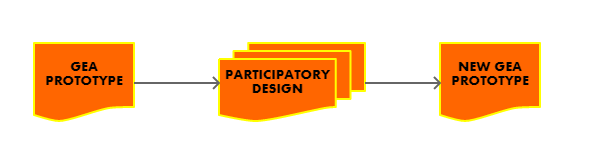
\includegraphics[width=12cm, height=4cm]{immagini/PD.png}
\caption{Phases of the work}\label{fig:phases}
\end{figure}

\section{GEA}
\subsection{Thesis Structure}
The thesis is organized as follows:
\begin{description}
\item[Chapter 2 (State of the art)] In this section we show all the technologies for Virtual Reality, explaining how they works and their relation with NDD people. We present also an instrument very useful for therapists that allows to replicate the smartphone's screen, Google Chromecast, and the touch screen evolution. Finally we describe the projects already developed about food education.
\item[Chapter 3 (GEA: first prototype)] Here we describe how we elicitate the requirements, which are our target groups, context, needs, constraints, goals. After that we show the UX design with description of all the app's pages and respective screenshot and flow diagram. Finally, we briefly describe the implementation overview.
\item[Chapter 4 (First evaluation)]  
\item[Chapter 5 (GEA: second prototype)]
\item[Chapter 6 (Second evaluation)] 
\item[Chapter 7 (Value proposition)]
\item[Chapter 8 (Challenges)]  
\item[Chapter 9 (Implementation)] We present all the tools used to build up our application and the hardware and software architecture description.
\item[Chapter 10 (Conclusion)]
\end{description}
At the end of the thesis, two appendices illustrate the materials used during the process
and show some pictures of the process.
 
\subsection{Origin of the name and mascotte}
We decide to give the name GEA to our application because of two reasons. The first one is that Gea, in the greek mythology, was the personification of the Earth, the mother of all life so she is also the symbol of the nature that recalls the nutrition's topic. The second motivation is that in Italian Gea is the acronym of "Gioco Educazione Alimentare", which translated is "Food Education Game", in this way in the title there is the objective's explanation.\\
We have also designed a mascotte depicting a fairy of fruit and vegetables to leak the message that even the characters recognized by the community as positive eat healthy food; it is in fact dressed with elements such as strawberries like pigtails, pumpkin like a skirt, salad like top and cherries like little bows of shoes.
\begin{figure}[H]
\centering
\begin{minipage}[c]{.40\textwidth}
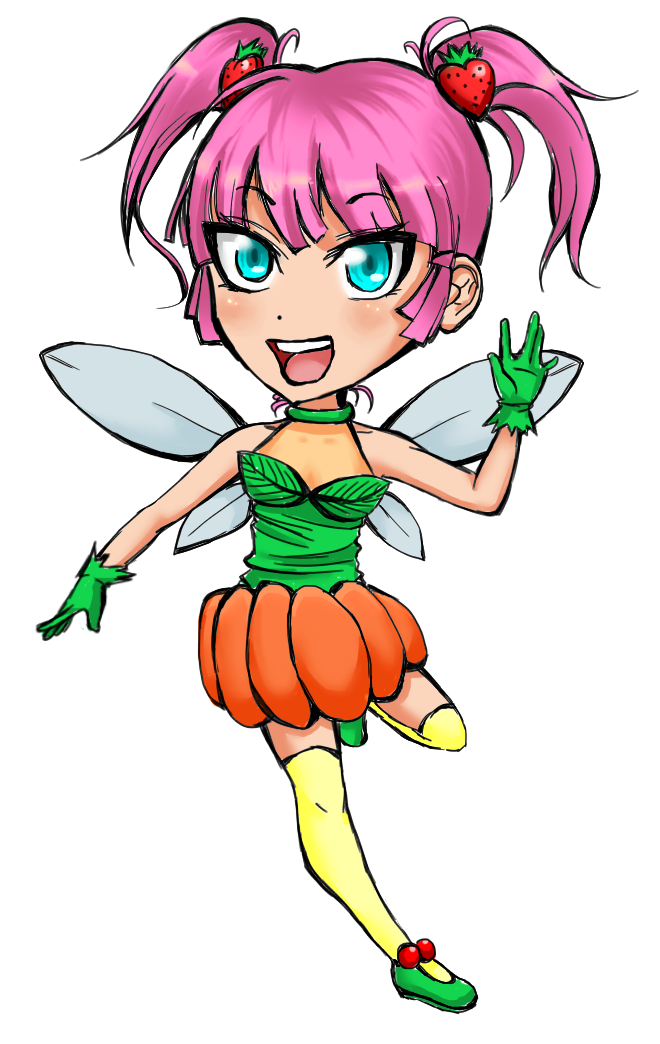
\includegraphics[width=1\textwidth]{immagini/geamasc.png}
\end{minipage}%
\hspace{10mm}%
\begin{minipage}[c]{.40\textwidth}

\includegraphics[width=1\textwidth]{immagini/GEA.png}
\end{minipage}
\caption{GEA logo and mascotte}\label{fig:logo}
\end{figure}